% section
\section{Image Prediction Architectures} \label{section::related}
 This section will describe a range of state-of-the-art architectures for image prediction. Image prediction is a very broad field, but almost all state-of-the-art solutions
 for image prediction share one common part, the recurrent module. LSTM's are the most used modules in image prediction, as they are able to store information over a long period of time, despite
 the standard RNN (recurrent neural network). All algorithms described here have a different way to perform image prediction, but all use a type of LSTM to store the time-series information.
 It is very common for this type of papers, that the authors start their experiments by using a synthetic dataset, in the most cases this is MovingMNIST \cite{LeCun1998} and then afterwards performing
 tests on natural images. For natural images, the authors often use action-recognition datasets, because the camera is fixed and only objects/people in the scenery are moving. Another approach
 is using natural image datasets, where the camera is also moving through the scenery, for example Kitti dataset \cite{Geiger2013}. This dataset consists of natural images from different car
 drives through the city and residential area of Karlsruhe. Therefore not only objects in the scenery are moving, but also the camera has a self-motion, which can be very tricky for image prediction
 algorithms to predict.
 
 % subsection
 \subsection{LSTM Autoencoder} \label{subsection::lstm_autoencoder}
  The paper \glqq Unsupervised Learning of Video Representations using LSTMs\grqq by Srivastava et. al. \cite{Srivastava2015} is using the standard LSTM~\ref{subsection::lstm} in an autoencoder
  architecture~\ref{subsection::autoencoder} for image reconstruction and future image prediction.
  The architecture is often used as a baseline in newer and more advanced architectures, because it consists of the standard LSTM as recurrent module.
  Due to the fact, that the LSTM module is not able to handle multi-dimensional data as is, the images need to be vectorized. The authors use
  MovingMNIST \cite{LeCun1998} as synthetic dataset, where every image is of size $64 \times 64 \times 1$. Therefore the image is vectorized into $64 \cdot 64 \times 1$ $=$ $4096 \times 1$.
  This MovingMNIST implementation consists of two digits inside every frame. The authors input $10$ images and output the next $10$ images.
  The model is end-to-end differentiable and trained using BPTT (backpropagation through time) \cite{Werbos1990}.
  For the synthetic dataset, the model is trained using cross-entropy loss with logits~\ref{subsection::pytorch}, for natural image
  datasets with MSE (mean-squared error) \cite{Zhao2017}.
  \begin{figure}[H]
   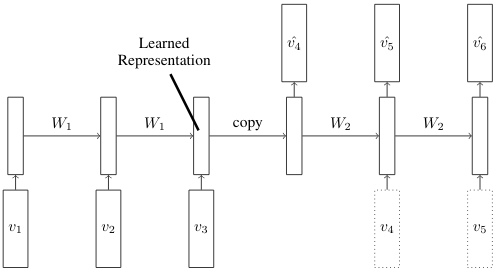
\includegraphics[width=0.45\textwidth]{../Images/srivastava.png}
   \centering
   \caption{Architecture for future image prediction \cite{Srivastava2015}}
   \label{fig:lstm_architecture}
  \end{figure}
  \begin{figure}[H]
   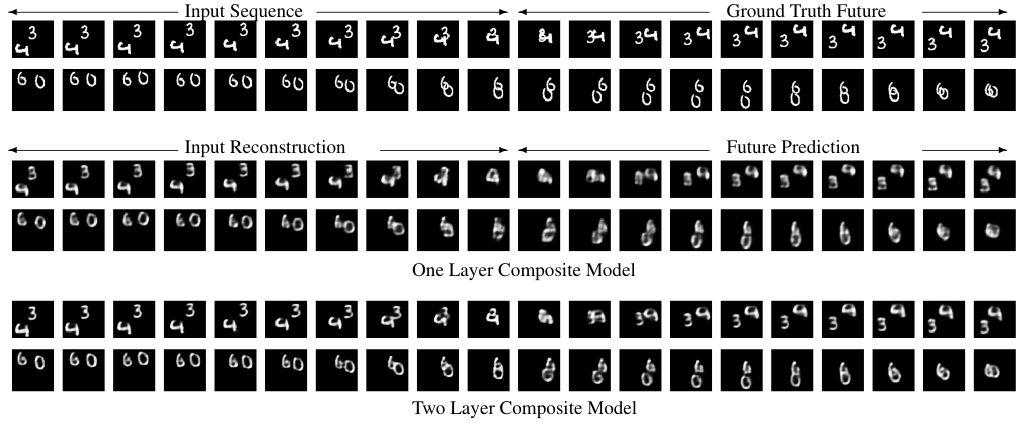
\includegraphics[width=0.85\textwidth]{../Images/srivastava_results_mnist.png}
   \centering
   \caption{Results for MovingMNIST \cite{Srivastava2015}}
   \label{fig:lstm_results}
  \end{figure}

 % subsection
 \subsection{ConvLSTM Autoencoder} \label{subsection::convlstm_autoencoder}
  The paper \glqq Convolutional LSTM Network: A Machine Learning Approach for Precipitation Nowcasting\grqq by Shi et. al. \citep{Shi2015} is using a similar architecture as Srivastava et. al. in
  section~\ref{fig:lstm_architecture}, but instead of using the standard LSTM, they use a novel ConvLSTM~\ref{subsection::convlstm}. The ConvLSTM used in this architecture is with 
  peephole~\ref{subsection::convlstm_peephole}.
  This architecture outperforms the implementation of Srivastava et. al., because it \glqq captures spatiotemporal correlations better\grqq.
  This model is, same as LSTM Autoencoder~\ref{subsection::lstm_autoencoder} end-to-end differentiable and trained using BPTT. It also uses the cross-entropy loss with logits for the synthetic dataset 
  (MovingMNIST) experiment. In this MovingMNIST implementation, every frame consists of three digits. As in the architecture above, the authors here input $10$ images and output $10$.
  \begin{figure}[H]
   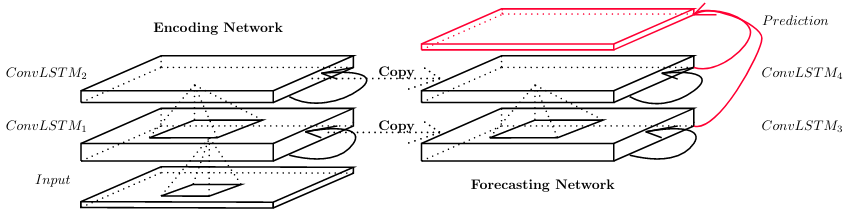
\includegraphics[width=0.65\textwidth]{../Images/shi.png}
   \centering
   \caption{Future image prediction model \cite{Shi2015}}
   \label{fig:convlstm_architecture}
  \end{figure}
  \begin{figure}[H]
   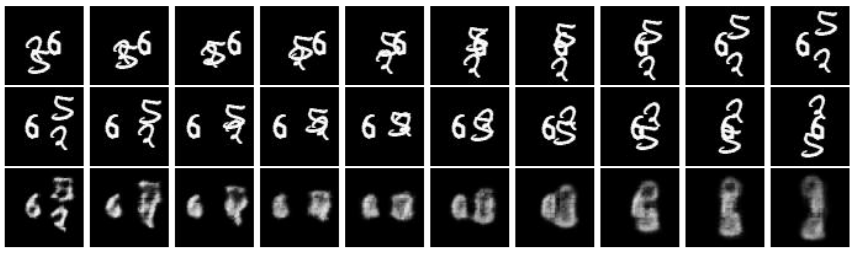
\includegraphics[width=0.5\textwidth]{../Images/shi_results_mnist.png}
   \centering
   \caption{Results for MovingMNIST. \textbf{First Row:} 10 input images, \textbf{Second Row:} Ground truth next images, \textbf{Third Row:} Prediction of 3-layer implementation \cite{Shi2015}}
   \label{fig:convlstm_results}
  \end{figure}
 
 % subsection
 \subsection{Spatio-temporal Video Autoencoder}
  The paper \glqq Spatio-temporal Video Autoencoder With Differentiable Memory\grqq by Patraucean et. al. \cite{Patraucean2015} describes a more complex architecture, in which the authors
  nest a temporal autoencoder inside a spatial autoencoder. The spatial autoencoder is a simple undercomplete autoencoder~\ref{subsection::autoencoder}, where the decoder uses nearest-neighbor
  upsampling to get the output image size correct. The temporal autoencoder consists of a ConvLSTM (A ConvLSTM without peephole~\ref{subsection::convlstm_nopeephole}, which works as the temporal 
  encoder and and an optical flow convolutional module, which works
  as the temporal decoder. The network idea is to insert the image sequence $X$, which will create an optical flow map. This optical flow map is then applied on the last given image, to shift every
  pixel to it's new position. This will create the next image. The idea behind this is given in \glqq Spatial Transformer Networks\grqq by Jadeberg et. al. \cite{Jadeberg2015}.
  The model is end-to-end differentiable and trained using BPTT. The authors also used MovingMNIST as synthetic dataset and use the cross-entropy loss with logits as reconstruction error for it. The 
  MovingMNIST implementation is the same as in LSTM Autoencoder~\ref{subsection::lstm_autoencoder} (With two digits per frame.).
  In contrast to the other algorithms, this architecture is only capable of doing one-frame prediction as is. The authors input $19$ images and output $1$ image.
  \begin{figure}[H]
   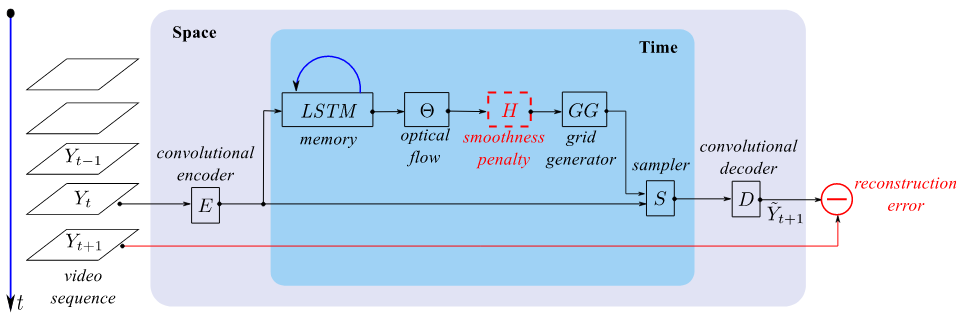
\includegraphics[width=0.65\textwidth]{../Images/patraucean.png}
   \centering
   \caption{Spatio-temporal Video Autoencoder \cite{Patraucean2015}}
   \label{fig:spatiotemp_architecture}
  \end{figure}
  \begin{figure}[H]
   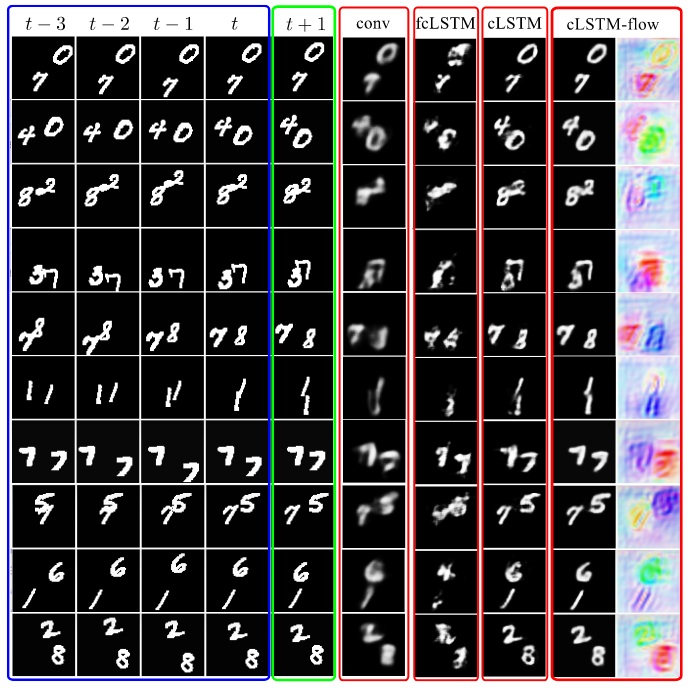
\includegraphics[width=0.5\textwidth]{../Images/patraucean_results_mnist.png}
   \centering
   \caption{Results for MovingMNIST. \textbf{conv:} Is a simple convolutional autoencoder, without recurrent module, \textbf{fcLSTM:} LSTM Autoencoder~\ref{subsection::lstm_autoencoder},
   \textbf{cLSTM:} ConvLSTM Autoencoder~\ref{subsection::convlstm_autoencoder}, \textbf{cLSTM-flow:} Spatio-temporal Video Autoencoder with extra output of flow-map. \cite{Patraucean2015}}
   \label{fig:spatiotemp_results}
  \end{figure}
 
 % subsection
 \subsection{PredNet}
  The paper \glqq Deep Predictive Coding Networks For Video Prediction And Unsupervised Learning\grqq by Lotter et. al. \cite{Lotter2016} composes an architecture, which is informally named
  \textbf{PredNet}. It describes a network architecture based on the concept of \glqq predictive coding\grqq \cite{Rao1999}, \cite{Friston2005}.
  \begin{figure}[H]
   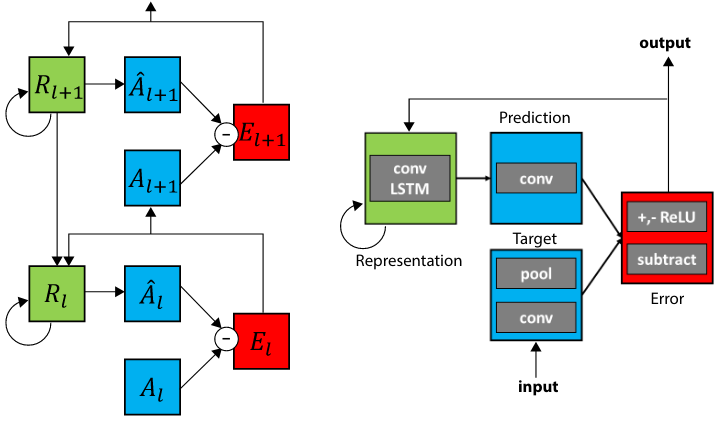
\includegraphics[width=0.65\textwidth]{../Images/lotter.png}
   \centering
   \caption{PredNet \cite{Lotter2016}}
   \label{fig:lotter_architecture}
  \end{figure}
 
 
  The chosen implementation for the experiments~\ref{section::experiments}.
